\chapter{Přílohy}
	%lze odebrat zobrazování jednotlivých příloh v obsahu
	%\addtocontents{toc}{\protect\setcounter{tocdepth}{0}}
	\section{Schéma databáze}
	\begin{figure}[hbtp]
		\centering %% příkaz, který ti obrázek zarovná na střed
		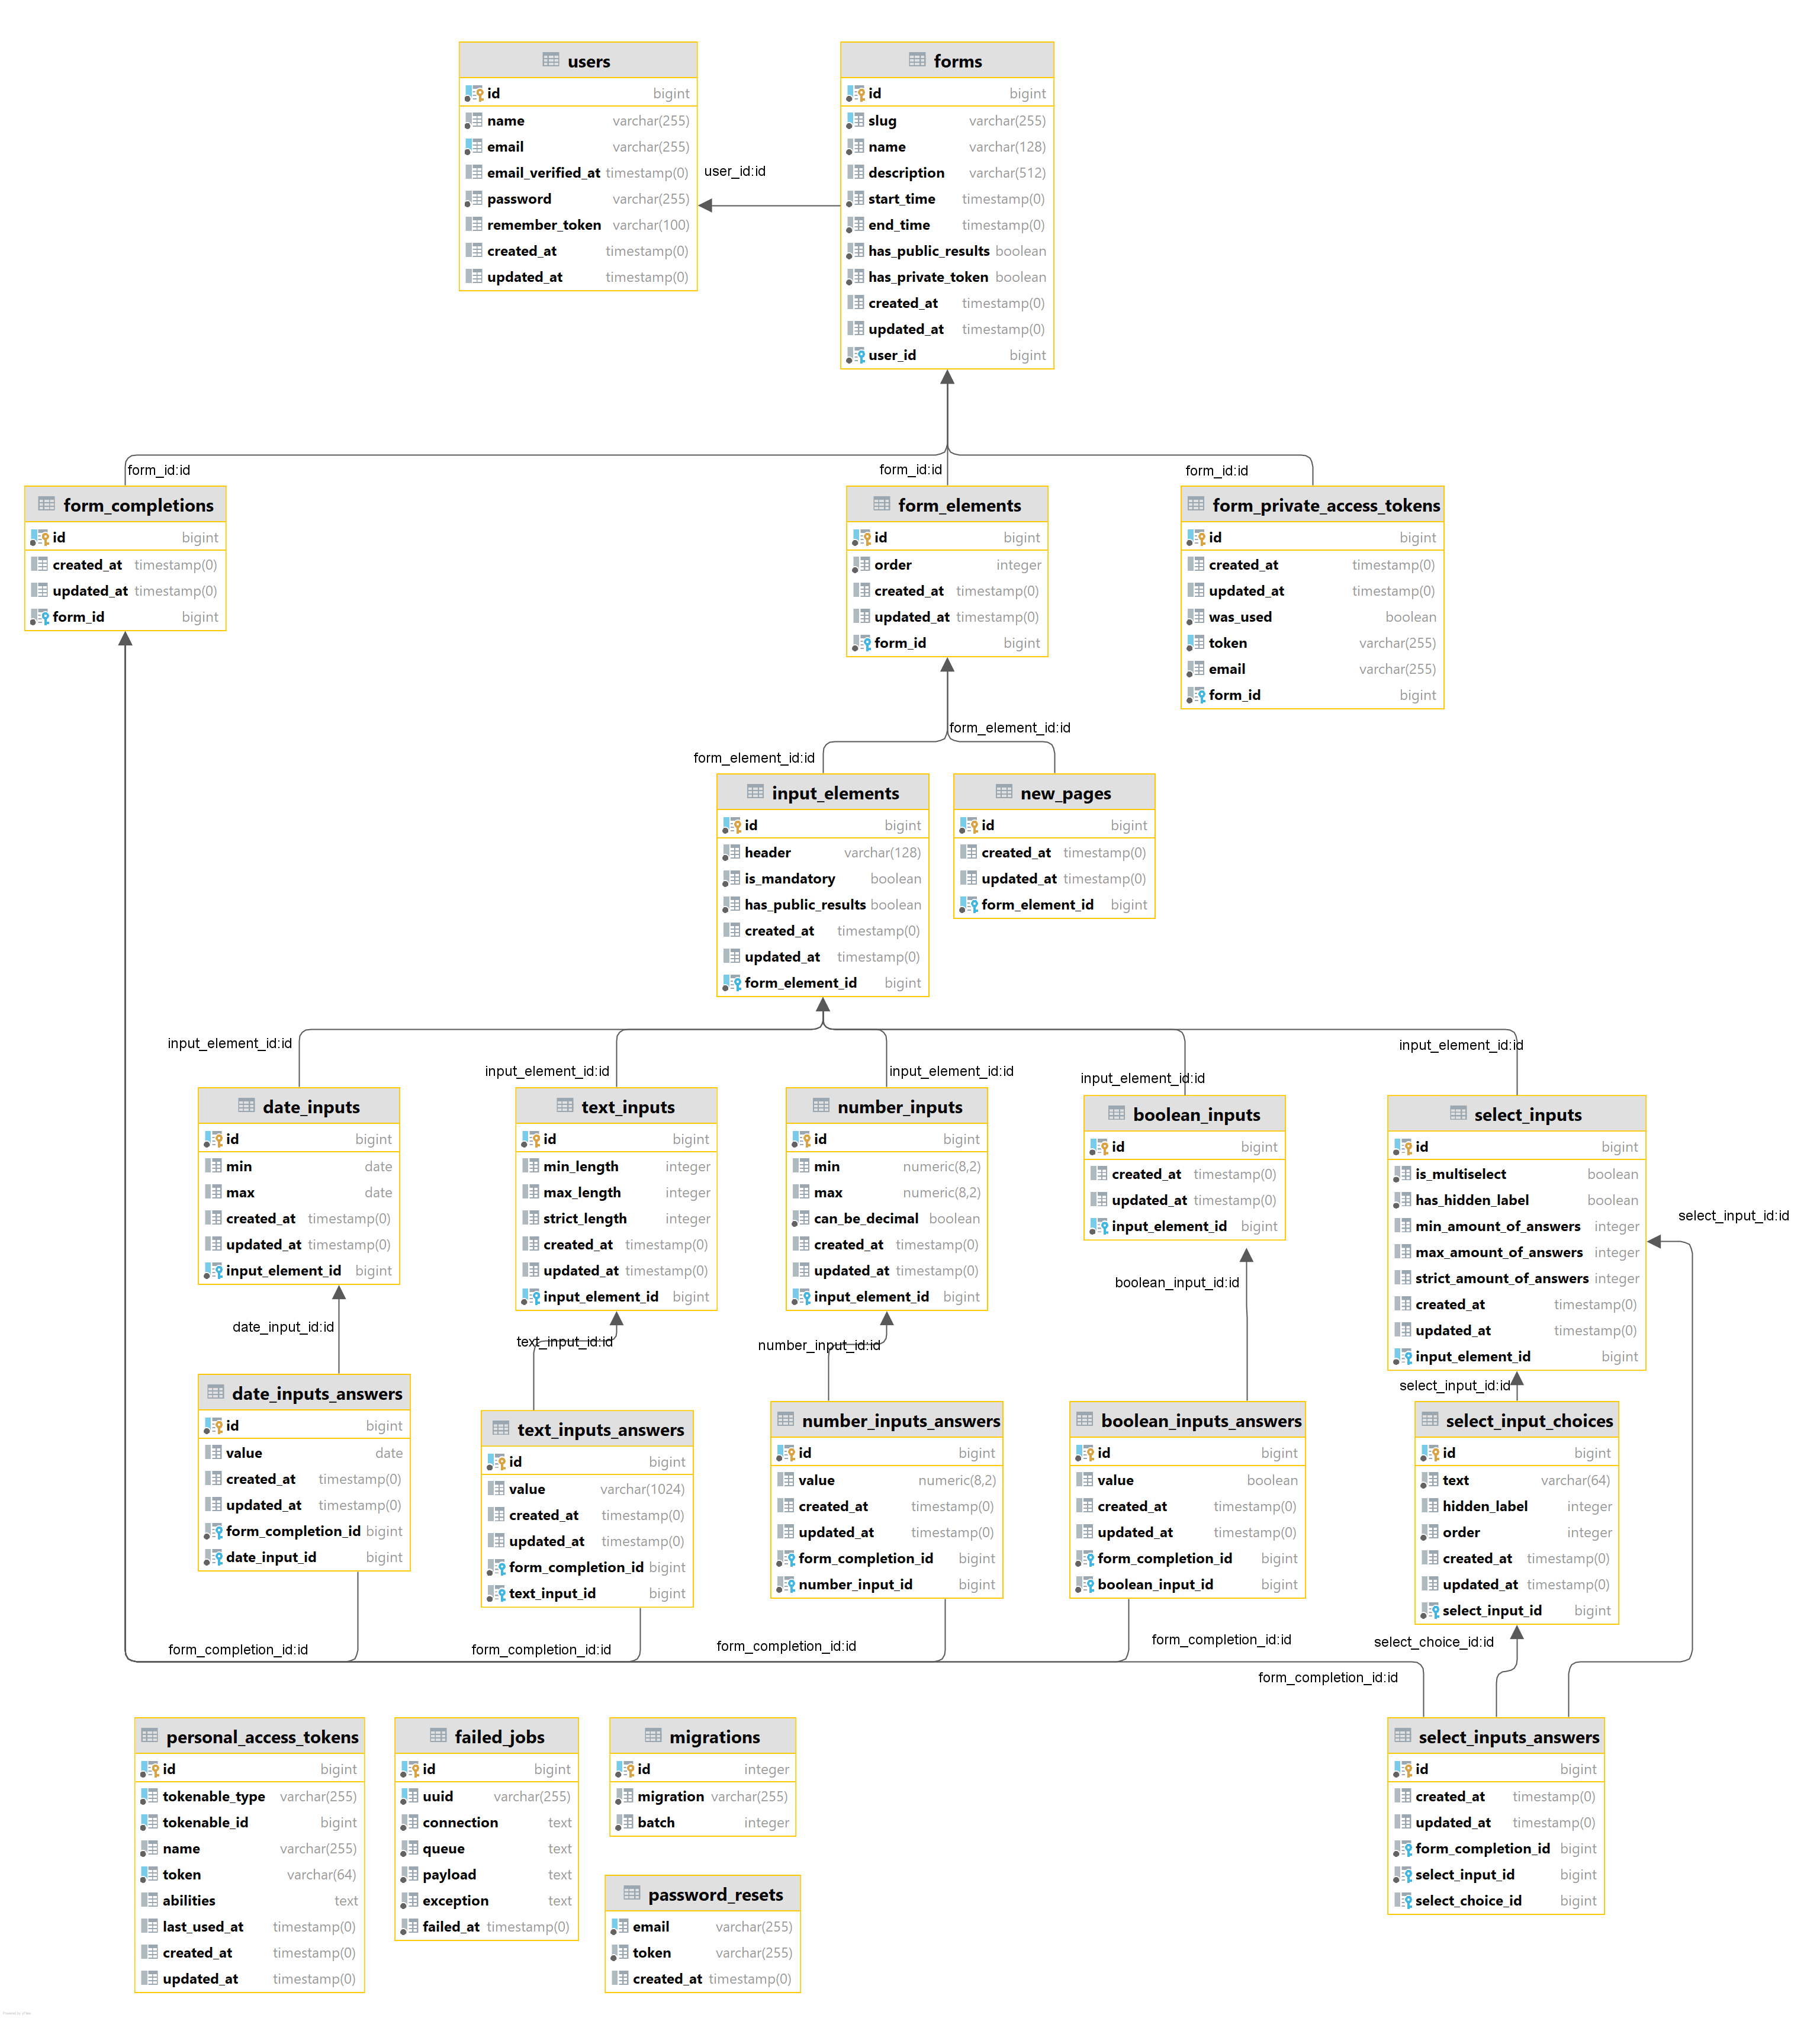
\includegraphics[height=0.61\paperheight]{img/db_diagram.png} %% vložení samotného obrátku
		\label{fig:db_diagram} %% označení až budeš chtít na obrázek odkazovat
	\end{figure}

	\newpage
	
	%\addtocontents{toc}{\protect\setcounter{tocdepth}{2}}

	